\chapter{One-Sample Confidence Intervals on a Mean When the Population Variance is Unknown}
\section{CIs for \(\mu\)}
\begin{definition}[Large-Sample Confidence Interval for \(\mu\)]

Let \(\mu\) be the population mean. When the population standard deviation \(\sigma\) is known and the sample size is large, a confidence interval for \(\mu\) is given by:
\[
\bar{Y} \pm z_{\alpha/2} \left( \frac{\sigma}{\sqrt{n}} \right)
\]
This interval is valid under the following conditions:
\begin{itemize}
  \item The sample is random.
  \item The observations are independent and identically distributed (i.i.d).
  \item The sample size \(n\) is large enough for the Central Limit Theorem (CLT) to apply.
\end{itemize}
\end{definition}

\begin{definition}[Small-Sample Confidence Interval for \(\mu\)]


Let \(\mu\) be the population mean. When the population standard deviation is unknown and the sample size is small, a confidence interval for \(\mu\) is given by:
\[
\bar{Y} \pm t_{\alpha/2} \left( \frac{S}{\sqrt{n}} \right), \quad \nu = n - 1
\]
This interval is valid under the following conditions:
\begin{itemize}
  \item The observations are independent and identically distributed (i.i.d).
  \item The sample is random.
  \item The population \textbf{must} follow a Normal distribution (CLT does not apply).
\end{itemize}
\end{definition}
\subsection*{Independence Assumption}

The data values should be independent. There’s really no way to check independence of the data by looking at the sample, but we should think about whether the assumption is reasonable.
\subsection*{Randomization Condition}

The data arise from a random sample or suitably randomized experiment. Randomly sampled data — especially data from a Simple Random Sample — are ideal.
\begin{tcolorbox}[title=\textbf{Normal Population Assumption}, 
  colback=yellow!10, 
  colframe=black!45, 
  coltitle=black, 
  fonttitle=\bfseries,
  breakable]

\begin{itemize}
  \item For very small samples (\(n < 15\) or so), the data should follow a Normal model pretty closely. If you do find outliers or strong skewness, don’t use this method.
  
  \item For moderate samples (\(n\) between 15 and 40 or so), the t-method will work well as long as the data is unimodal and reasonably symmetric. Make a histogram, boxplot, or Q–Q plot to check.
  
  \item When the sample size is larger than 40 or 50, the t-method is safe to use unless the data are extremely skewed. Make a histogram, boxplot, or Q–Q plot to check.
\end{itemize}

\end{tcolorbox}
\subsection*{Standard Error}

When the standard deviation of a statistic is estimated from data, the result is called the \textit{standard error} of the statistic. The standard error of the sample mean \(\bar{x}\) is 
\[
\frac{s}{\sqrt{n}}.
\]
\begin{tcolorbox}[title=\textbf{The \textit{t} Distributions}, 
  colback=yellow!10, 
  colframe=black!45, 
  coltitle=black, 
  fonttitle=\bfseries,
  breakable]

\begin{itemize}
  \item The density curves of the \textit{t} distributions are similar in shape to the Standard Normal curve. They are symmetric about 0, single-peaked, and bell-shaped.

  \item The spread of the \textit{t} distributions is a bit greater than that of the Standard Normal distribution. The \textit{t} distributions have more probability in the tails and less in the center than the Standard Normal. This is because substituting the estimate \(s\) for the fixed parameter \(\sigma\) introduces more variation into the statistic.

  \item As the degrees of freedom increase, the \textit{t} density curve approaches the \(N(0, 1)\) curve more closely. This happens because \(s\) estimates \(\sigma\) more accurately as the sample size increases. So using \(s\) in place of \(\sigma\) causes little extra variation when the sample is large.
\end{itemize}

\end{tcolorbox}
\begin{figure}[H]
  \centering
  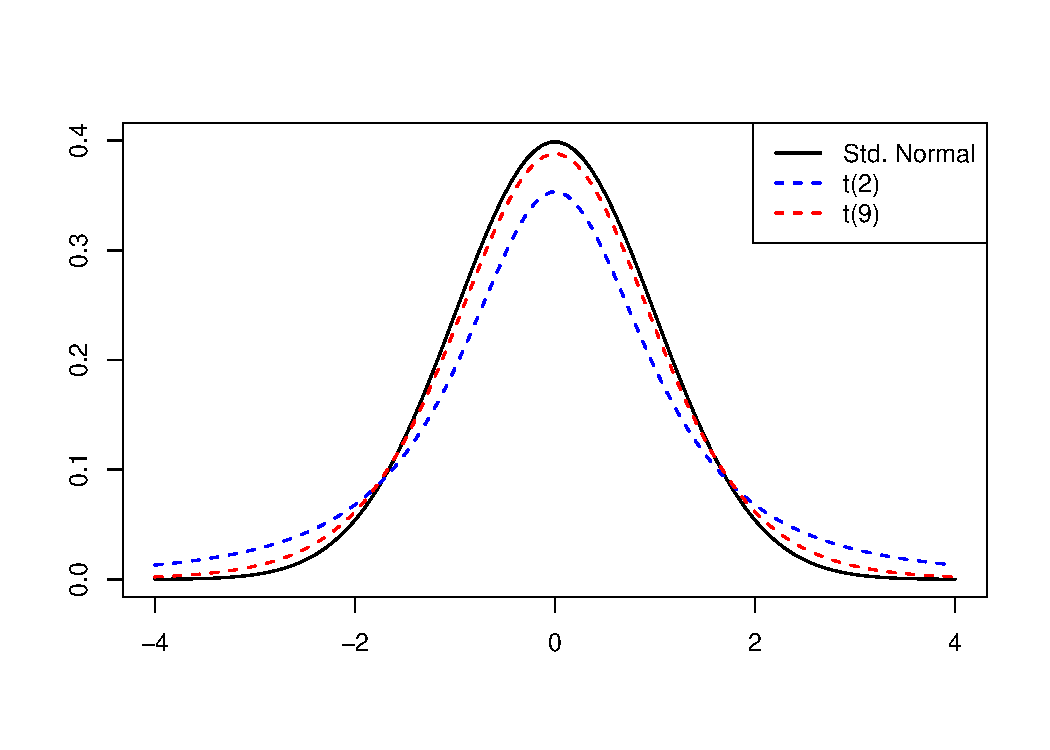
\includegraphics[width=0.8\textwidth]{section7/images/density_curves.pdf}
 \vspace{-2em} % Tweak until tight but not overlapping
  \caption{Comparison of the standard normal distribution and t-distributions with 2 and 9 degrees of freedom.}
  \label{fig:density-curves}
\end{figure}
\begin{example}[Ancient Air]

The composition of the Earth's atmosphere may have changed over time. To study the nature of the atmosphere long ago, scientists examined the gas in air bubbles trapped in ancient amber. Amber is fossilized tree resin that preserved the atmospheric gases at the time it was formed.

Measurements on amber specimens from the late Cretaceous era (75 to 95 million years ago) give the following percent values of nitrogen:

\begin{center}
63.4, 65.0, 64.4, 63.3, 54.8, 64.5, 60.8, 49.1, 51.0
\end{center}

Assume these observations are a simple random sample (SRS) from the population of all ancient air bubbles. Construct a \textbf{90\% confidence interval} to estimate the mean percent of nitrogen in ancient air. (Today’s atmosphere contains about 78.1\% nitrogen.)

\vspace{1em}
\textbf{Solution:}

Let \(\mu\) represent the true mean percent of nitrogen in ancient air. We compute a 90\% confidence interval for \(\mu\) using the sample data.

Given: 
\[
\bar{x} = 59.5888, \quad s = 6.2552, \quad n = 9, \quad t^* = 1.860 \quad (\text{df} = 8)
\]

\[
59.5888 \pm 1.860 \left( \frac{6.2552}{\sqrt{9}} \right) = 59.5888 \pm 3.8782
\]

\[
\boxed{55.7106 \text{ to } 63.4670}
\]

\vspace{1em}
\noindent\textbf{R code:}

\begin{tcolorbox}[colback=gray!10, colframe=black!45, arc=2mm]

\begin{verbatim}
# Step 1: Entering the data
nitrogen <- c(63.4, 65.0, 64.4, 63.3, 54.8, 64.5, 60.8, 49.1, 51.0)

# Step 2: Constructing the 90% confidence interval
t.test(nitrogen, conf.level = 0.90)
\end{verbatim}
\end{tcolorbox}

\vspace{1em}
\noindent\textbf{R output:}

\begin{tcolorbox}[colback=gray!10, colframe=black!45, arc=2mm]
\begin{verbatim}
One Sample t-test

data:  nitrogen
t = 28.578, df = 8, p-value = 2.43e-09
alternative hypothesis: true mean is not equal to 0
90 percent confidence interval:
 55.71155 63.46622
sample estimates:
mean of x 
  59.58889 
\end{verbatim}
\end{tcolorbox}

\end{example}
\begin{example}[Digital Camera Storage]

Most owners of digital cameras store their pictures on the camera. Some will eventually download these to a computer or print them using their own printers or a commercial printer. A film-processing company wanted to know how many pictures were stored on cameras.

A random sample of 10 digital camera owners produced the following data:

\begin{center}
25, 6, 22, 26, 31, 18, 13, 20, 14, 2
\end{center}

Estimate with \textbf{95\% confidence} the mean number of pictures stored on digital cameras.


---

\textbf{Solution:}

We are given raw data with \(n = 10\) and no information about the population standard deviation, so we construct a confidence interval for the population mean using the t-distribution.

\vspace{1em}
\textbf{Step 1: Compute sample statistics}

\begin{itemize}
  \item Sample mean: \(\bar{x} = \dfrac{177}{10} = 17.7\)
  \item Sample variance (method 1 – direct): 
  \[
  s^2 = \dfrac{\sum (x_i - \bar{x})^2}{n - 1} = \dfrac{742}{9} = 82.4556
  \]
  \item Sample standard deviation:
  \[
  s = \sqrt{82.4556} = 9.081
  \]
\end{itemize}

\vspace{1em}
\textbf{Step 2: Find the critical value}

For a 95\% confidence interval with \(n = 10\), degrees of freedom = 9. From the t-distribution table:
\[
t_{(9, 0.025)} = 2.262
\]

\vspace{1em}
\textbf{Step 3: Construct the confidence interval}

\[
\bar{x} \pm t^* \cdot \dfrac{s}{\sqrt{n}} = 17.7 \pm 2.262 \cdot \dfrac{9.081}{\sqrt{10}} = 17.7 \pm 6.495
\]

\[
\boxed{11.205 \text{ to } 24.195}
\]

\vspace{1em}
\textbf{Interpretation:}

We are 95\% confident that the mean number of images stored on digital cameras is between 11.205 and 24.195.

---

\noindent\textbf{R code:}

\begin{tcolorbox}[colback=gray!10, colframe=black!45, arc=2mm]
\begin{verbatim}
# Step 1: Entering data
dataset <- c(25, 6, 22, 26, 31, 18, 13, 20, 14, 2)

# Step 2: Finding 95% confidence interval
t.test(dataset, conf.level = 0.95)
\end{verbatim}
\end{tcolorbox}

\noindent\textbf{R output:}

\begin{tcolorbox}[colback=gray!10, colframe=black!45, arc=2mm]
\begin{verbatim}
One Sample t-test

data:  dataset
t = 6.164, df = 9, p-value = 0.0001659
alternative hypothesis: true mean is not equal to 0
95 percent confidence interval:
 11.2042 24.1958
sample estimates:
mean of x 
     17.7 
\end{verbatim}
\end{tcolorbox}
\end{example}
\begin{example}[Electric Insulators]

A manufacturing company produces electric insulators. If the insulators break when in use, a short circuit is likely. To test the strength of the insulators, destructive testing is performed to determine how much force (in pounds) is required to break them.

The following dataset consists of force values (in pounds) recorded for a random sample of 30 insulators:

\begin{center}
\noindent\ttfamily
1870, 1728, 1656, 1610, 1634, 1784, 1522, 1696, 1592, 1662, 1866, 1764, 1734, 1662, 1734, 1774, 1550, 1756, 1762, 1866, 1820, 1744, 1788, 1688, 1810, 1752, 1680, 1810, 1652, 1736
\end{center}

Construct a \textbf{95\% confidence interval} for the population mean force required to break the insulators.



 \textbf{Solution:}

We want a confidence interval for the population mean \(\mu\), where \(\mu =\) mean force required to break electric insulators. The population standard deviation is unknown, so we use a \textit{one-sample} t-interval.

\vspace{1em}
\noindent\textbf{R code:}

\begin{tcolorbox}[colback=gray!10, colframe=black!45, arc=2mm]



\begin{verbatim}
# Step 1. Entering data;
dataset <- c(1870, 1728, 1656, 1610, 1634, 1784, 1522, 1696, 1592, 1662,
             1866, 1764, 1734, 1662, 1734, 1774, 1550, 1756, 1762, 1866,
             1820, 1744, 1788, 1688, 1810, 1752, 1680, 1810, 1652, 1736)

# Step 2. Finding CI;
t.test(dataset, conf.level = 0.95)
\end{verbatim}
\end{tcolorbox}

\vspace{1em}
\noindent\textbf{R output:}

\begin{tcolorbox}[colback=gray!10, colframe=black!45, arc=2mm]



\begin{verbatim}
One Sample t-test

data:  dataset
t = 105.41, df = 29, p-value < 2.2e-16
alternative hypothesis: true mean is not equal to 0
95 percent confidence interval:
 1689.961 1756.839
sample estimates:
mean of x 
   1723.4 
\end{verbatim}
\end{tcolorbox}

\vspace{1em}
\textbf{Interpretation:}

We are 95\% confident that the average force required to break an electric insulator is between \textbf{1689.961 pounds} and \textbf{1756.839 pounds}.
\end{example}
\begin{example}[Assembly Time Estimation]

The operations manager of a production plant would like to estimate the mean amount of time a worker takes to assemble a new electronic component. After observing 120 workers assembling similar devices, she noticed that their average time was 16.2 minutes (with a standard deviation of 3.6 minutes).

Construct a \textbf{92\% confidence interval} for the mean assembly time. State all necessary assumptions.

\end{example}
\begin{example}[Tax Collected from Audited Returns]

In 2010, 142,823,000 tax returns were filed in the United States. The Internal Revenue Service (IRS) examined 1.107\%, or 1,581,000, of them to determine if they were correctly done. To evaluate auditor performance, a random sample of these returns was drawn and the additional tax was recorded.

Estimate with 95\% confidence the mean additional income tax collected from the 1,581,000 files audited.\\



\textbf{Solution:}

We use a one-sample confidence interval for the population mean additional tax collected.

\textbf{Step 1: Import the data from \texttt{taxes.txt}}

\begin{tcolorbox}[colback=gray!10, colframe=black!45, arc=2mm]
\begin{verbatim}

# url of taxes;
url <- "https://mcs.utm.utoronto.ca/~nosedal/data/taxes.txt"
taxes_data <- read.table(url, header = TRUE)

# inspect structure
names(taxes_data)
head(taxes_data)

# isolate the tax values
taxes <- taxes_data$Taxes
\end{verbatim}
\end{tcolorbox}

\vspace{1em}
\textbf{Step 2: Plot the data}

\textit{Histogram:}
\begin{tcolorbox}[colback=gray!10, colframe=black!45, arc=2mm]
\begin{verbatim}
hist(taxes,
     main = "Histogram for our example",
     xlab = "taxes", ylab = "frequency",
     col = "blue")
\end{verbatim}
\end{tcolorbox}

\begin{center}
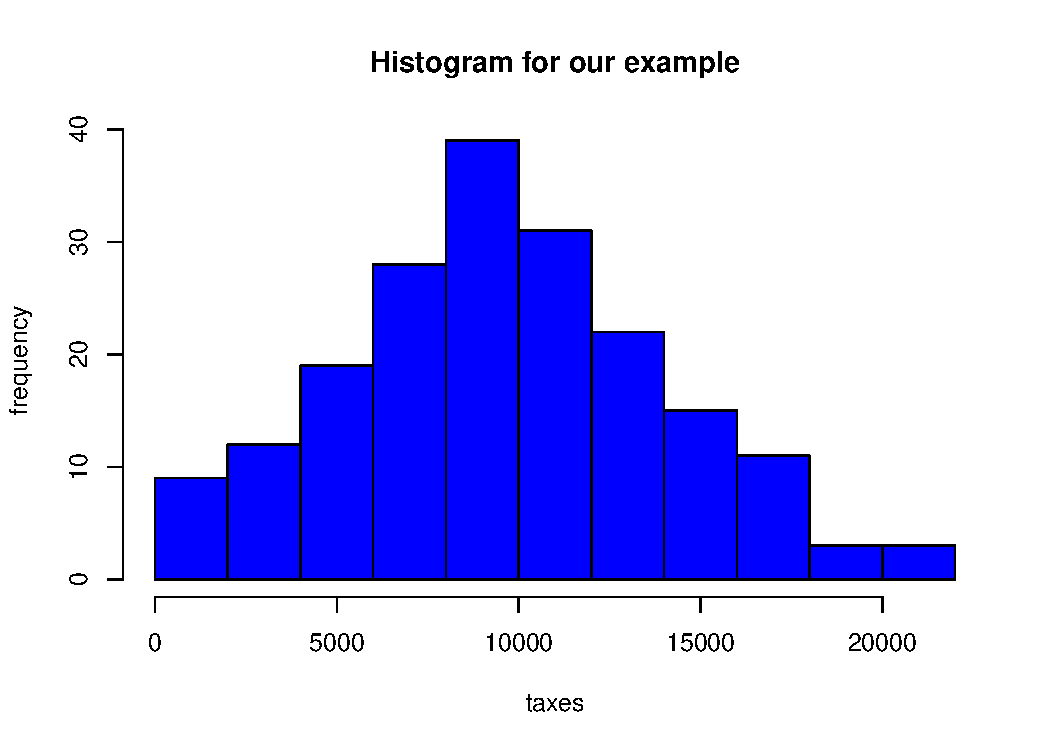
\includegraphics[width=0.6\textwidth]{Section7/images/tax_histogram.pdf}
\end{center}

\textit{Boxplot:}

\begin{tcolorbox}[colback=gray!10, colframe=black!45, arc=2mm]
\begin{verbatim}
boxplot(taxes,
        main = "Additional Income Tax",
        col = "blue")
\end{verbatim}
\end{tcolorbox}

\begin{center}
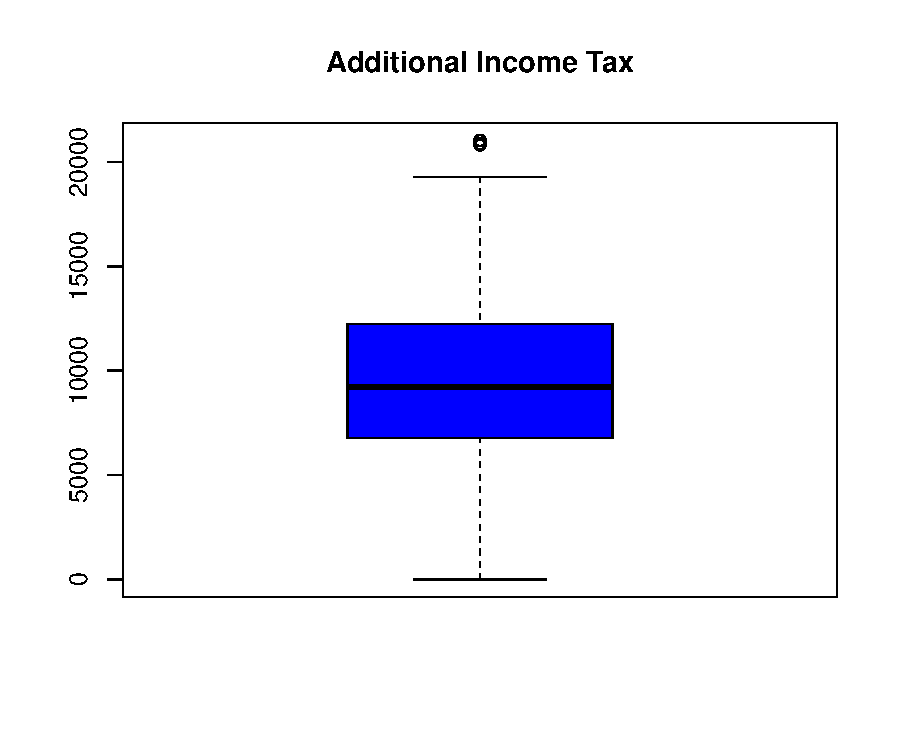
\includegraphics[width=0.5\textwidth]{Section7/images/tax_boxplot.pdf}
\end{center}

\textit{Q-Q Plot:}

\begin{tcolorbox}[colback=gray!10, colframe=black!45, arc=2mm]

\begin{verbatim}
qqnorm(taxes, col = "blue", pch = 19)
qqline(taxes)
\end{verbatim}
\end{tcolorbox}

\begin{center}
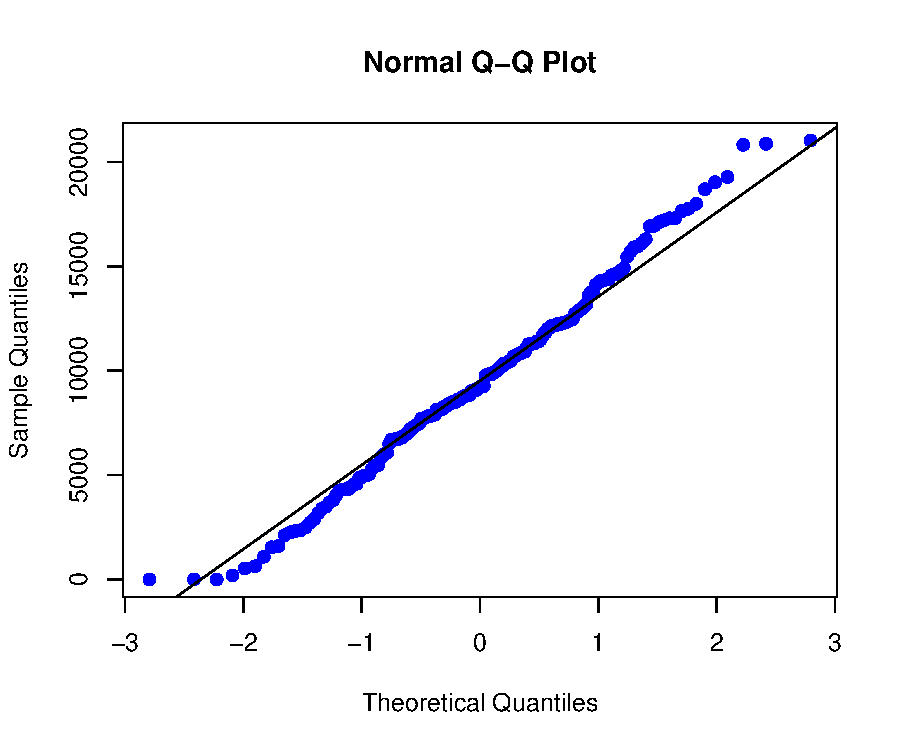
\includegraphics[width=0.55\textwidth]{Section7/images/tax_qqplot.pdf}
\end{center}

\vspace{1em}
\textbf{Step 3: Construct 95\% CI}

\begin{tcolorbox}[colback=gray!10, colframe=black!45, arc=2mm]

\begin{verbatim}
t.test(taxes, conf.level = 0.95)
\end{verbatim}
\end{tcolorbox}

\vspace{0.5em}
\textbf{Interpretation:} Based on the t-test, we are 95\% confident that the average additional tax collected lies within the interval calculated from the sample.

\textbf{Assumptions:}
\begin{itemize}
  \item The sample is a random sample from the population of interest.
  \item Observations are independent.
  \item The population is approximately Normal, or the sample size is large enough (justified by the histogram, boxplot, and Q-Q plot).
\end{itemize}

\begin{tcolorbox}[colback=gray!10, colframe=black!45, arc=2mm]


\begin{verbatim}
## 
##  One Sample t-test
## 
##  data:  taxes
##  t = 29.345, df = 191, p-value < 2.2e-16
##  alternative hypothesis: true mean is not equal to 0
##  95 percent confidence interval:
##   8886.932 10167.721
##  sample estimates:
##  mean of x 
##    9527.326 
\end{verbatim}
\end{tcolorbox}

\bigskip

\textbf{Interpretation:}

We estimate that the mean additional tax collected lies between \$8,887 and \$10,168 (with 95\% confidence).
\end{example}
\subsection*{A few final comments}

When we introduced the Student \emph{t}-distribution, we pointed out that the \emph{t}-statistic is Student \emph{t}-distributed if the population from which we’ve sampled is Normal. However, statisticians have shown that the mathematical process that derived the Student \emph{t}-distribution is \textbf{robust}, which means that if the population is non-Normal, the results of the confidence interval estimate are still valid provided that the population is \textbf{not extremely non-Normal}. Our histogram, boxplot, and Q--Q plot suggest that our variable of interest is not extremely non-Normal, and in fact, may be Normal.


